\chapter{Introduction}
\label{chap:introduction}
Readers unfamiliar with the terms of relational-database normalization and 
functional dependencies can find a brief introduction on the subject in
Chapter~\ref{chap:preliminaries}. 

Due to its great importance for database applications database schema design has
attracted substantial research~\cite{p1}. Relational-database normalization is a 
theoretical approach for structuring a database schema and it is very well developed. 
Unfortunately, theory is not yet understood well by practitioners~\cite{p1}.
One of the reasons for this is the lack of good tools which could aid the students 
during the learning process of relational-database normalization~\cite{p8}. 
Thus our learning environment was developed in order to give students the ability to 
easily and efficiently test
their knowledge of the different normal forms in practice. The environment assists the students by 
providing them the following functionalities:

\begin{enumerate}
	\item Allow the student to specify a candidate decomposition of a given relation.
	\item Assess the correctness of the student's proposed decomposition relative to many factors; including:
		\begin{itemize}
			\item Lossless-join property.
			\item Dependency preservation.
			\item Specification of keys.
			\item Correctness of the Second Normal Form (2NF), Third Normal Form (3NF) and
			 Boyce-Codd Normal Form (BCNF) decompositions.
		\end{itemize}
	\item Provide students with sample decompositions when needed. 
	\item Allow users to communicate with each other via comments/posts.
\end{enumerate}

Our learning environment uses many different normalization 
algorithms for achieving the functionalities described above. 
We can divide them into two different groups:

\begin{description}
	\item[Decomposition algorithms] are used for decomposing a normalized database 
	schema into a certain normal form using functional dependencies (FDs).
	\item[Test algorithms] for testing whether a given relational schema
	violates certain normal form, the lossless-join property or other criteria.
\end{description}

A given schema may have many decompositions into a given normal form.
Therefore, simply computing one such decomposition and comparing the
student's solution to it is not satisfactory.  Rather, what is needed
are test algorithms which check a decomposition proposed by the student for
correctness.

Here it is worth mentioning that the normalization algorithms often require 
background in relational algebra that most IS/IT students lack~\cite{p8}. This
is also an issue which our tool addresses by providing a more intuitive 
way of decomposing a schema and by giving an easy way for lecturers to
teach by example and test the knowledge of their students. 

\section{Organization of This Report}
\label{sec:organization}
In the remaining sections of this chapter we introduce informally 
the key features and concepts of our web-based learning environment, 
called LDBN (Learn DataBase Normalization)~\cite{wldbn}; 
compare it to a couple of other 
available web-based database normalization tools, and provide the reader with small glossary.  
%The introduction to LDBN in Section~\ref{sec:introldbn} is important for the reader
%in order for him/her to better understand the need and the concepts of the algorithms described in 
In Chapter~\ref{chap:preliminaries} we give definitions to
relational-database normalization and to the different normal forms. 
In Chapter~\ref{chap:design} we discuss some design issues regarding LDBN such as 
platform choice and others. Chapter~\ref{chap:impl} provides a formal description
of our reference implementation of the learning environment, and
Chapter~\ref{chap:conclusion} shows our conclusions.

\section{Learning Database Normalization with LDBN}
\label{sec:introldbn}
In this section we briefly introduce our reference implementation
of the web-based learning environment, called LDBN.    
Figure~\ref{fig:screen01} shows the overview of the most important part of the user interface~(UI)~- 
the \textit{Solve Assignment} view/tab. Here students can test their knowledge on 
the subject of relational-database normalization. The first thing the reader 
may notice is the fact that LDBN runs within a browser. The client side 
of LDBN is written in JavaScript following the AJAX techniques 
(more about this in Chapter~\ref{chap:design}). 
Furthermore, LDBN is assignment driven. This means students have to first 
choose an assignment 
from a list with assignments, submitted by other users (lecturers). 
Such a list is shown in Figure~\ref{fig:screen02}. 
An assignment consists of a relational-database schema in
universal-relation form (URF), i.e., all the attributes in a single relation 
and a set of FDs on the attributes. 
After an assignment has been loaded, we require the students to go through the 
following steps in LDBN:
\begin{enumerate}
	\item Determine a minimal cover of the given FDs, also known as a canonical cover.
	\item Decompose the relational schema which is in URF into 2NF, 3NF and BCNF. 
	\item Determine a primary key for each new relation/table. 
\end{enumerate}

\begin{figure}[h]
	\begin{center}
		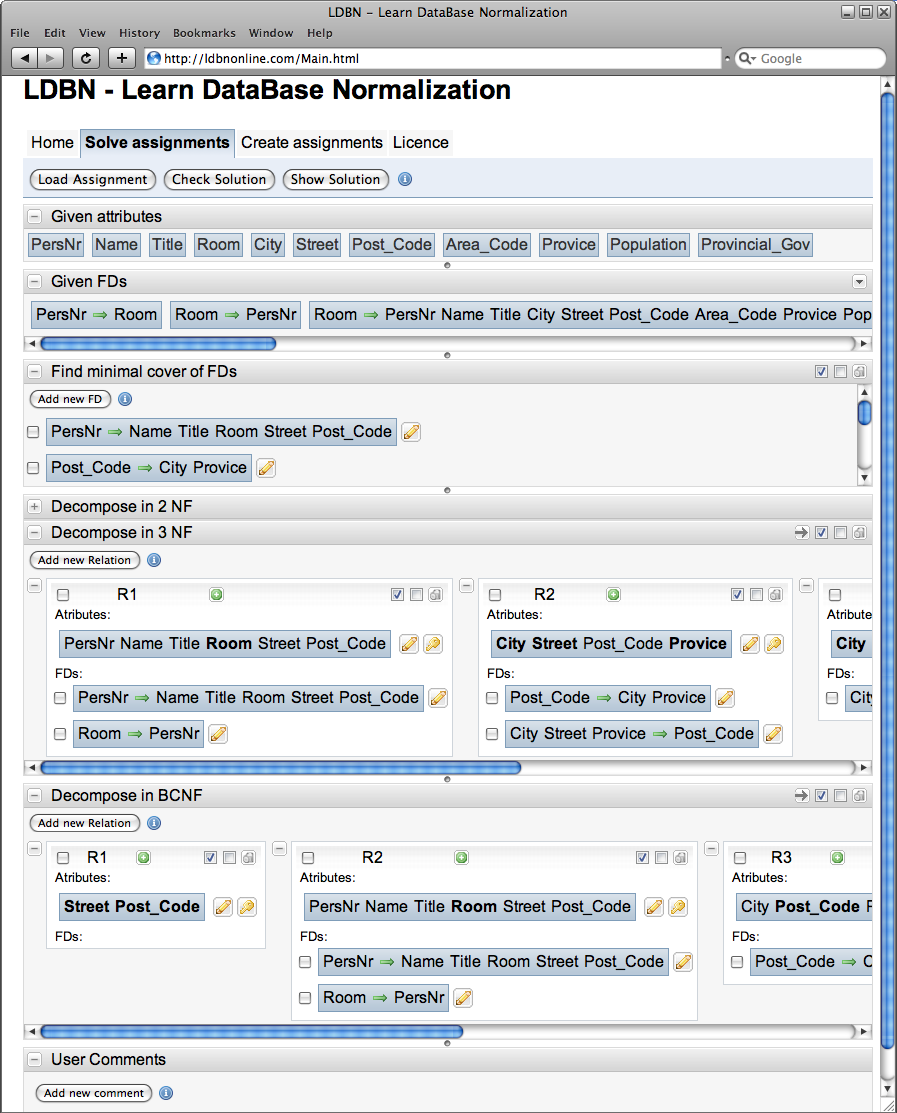
\includegraphics[width=0.8\textwidth]{./img/screen01b.png}
		\caption{Solve Assignments Tab}
		\label{fig:screen01}
	\end{center}
\end{figure}

\begin{figure}[h]
	\begin{center}
		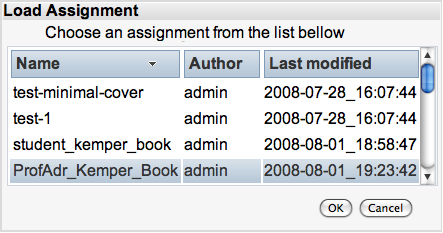
\includegraphics[width=0.6\textwidth]{./img/screen02.png}
		\caption{Load Assignments List}
		\label{fig:screen02}
	\end{center}
\end{figure}

The task of checking a potential solution
involves many subtasks, which may be performed in any order. In addition to this,  a partial or complete 
solution can be submitted at any given time by pressing the \textit{Check Solution} button. 
After that the system analyzes the solution by performing the following checks:
\begin{enumerate}
	\item Correctness of the minimal cover of the given FDs. 
	\item Correctness of the FDs associated with each relation $R$; that is, 
    if the FDs are actually in the embedded closure of $F_{R}\sp{+}$ for this relation. 
    See Section~\ref{sec:closureF} for more details on a closure of a set of FDs.   
	\item Losses-join properly for every schema in the decomposition.
	\item Dependency preservation for every decomposition.
	\item Correctness of the key of each relation.
	\item Correctness of the decomposition, i.e., if the decomposition is really in 2NF, 3NF and BCNF.
\end{enumerate}

\begin{figure}[h]
	\begin{center}
		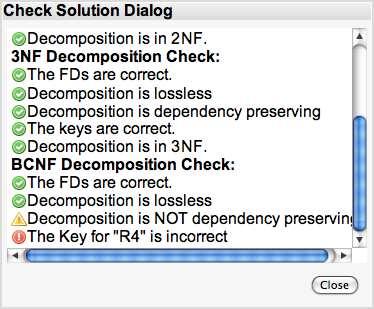
\includegraphics[width=0.6\textwidth]{./img/screen03a.png}
		\caption{Check Solution Dialog}
		\label{fig:screen03}
	\end{center}
\end{figure}

A dialog with the result is shown to the user. In case of an error the system offers
feedback in form of small textual hints, indicating
where the error might be. Such a dialog is shown in Figure~\ref{fig:screen03}. In this case
we can see that the user has made a correct decomposition for 2NF and 3NF,
but his/her decomposition for BCNF has some errors, namely the key of the relation R4 is
incorrect. The dialog shows that the decomposition does not 
satisfy the dependency-preservation property, but in the case of BCNF this
is not always possible, therefore it is only a warning. 

Additional features of LDBN include creating an assignment, which can be done 
only by registered users. This restriction is necessary in order users to be able 
to distinct assignments provided by trusted users, e.g. the database course
lecturers. Registered users have also the ability to leave textual comments 
for every assignment. On the one hand, such
comments ensure that user can easily communicate and share ideas
with each other, and one the other hand, comments could also decrease the amount of workload
for the lecturers in terms of giving an explanation to difficult decomposition.

More detailed and formal description of the features of LDBN will be given in
Chapter~\ref{chap:impl}. 

\section{Comparation of LDBN with Other Tools}
\label{sec:comparation}
In this section we compare LDBN to a couple of other 
available web-based database normalization tools 
such as the \textit{Web-based Tool to Enhance Teaching/Learning Database 
Normalization} by Kung~\cite{p8} and the \textit{The Database Normalization Tool}
\cite{w1}. Furthermore, we discuss why we think our tool is better 
and more efficient
in terms of teaching potential, and give possible reasons why the 
other tools are not commonly used by students.

First of all, the concept of assignments is a major
difference between LDBN and the other normalization tools, 
which only provide 
one possible solution (decomposition) to the user, without users having the ability to test 
themselves. On the other hand, LDBN can be used for checking the correctness of any
proposed decomposition. This could be useful for lectures to test handwritten assignments. 

Another major advantage of LDBN over the other tools is the user interface (UI). 
As Frye~\cite{p12} and Dantin~\cite{p9} stated, this is often a
neglected feature when it comes to educational software. The lack of user-friendly UI 
can often lead to unpopularity of the software among students. An example here could be 
\textit{The Database Normalization Tool}~\cite{w1}. Inputting a relational schema in the program can
take quite some time due to the fact that
users have to input every attribute manually using the keyboard and then also 
have to input every FD the same way. This may take several minutes even for small  
assignments. Furthermore, relational schemas cannot be saved for future use as 
in LDBN, and users have to input them again next time. To overcome this slow input of user data, 
LDBN supports drag and drop. A feature widely used in desktop
applications, but relatively new to an AJAX application such as LDBN. Every attribute
and every FD in LDBN can be dragged and dropped, in order 
to define or modify FDs, key attributes, etc. This ensures a really fast and easy
usage of the tool without the need for keyboard input. It should be mentioned
that inputting attributes the traditional way by typing them is also supported.

Community features such as posting comments are not present in the other two web-based 
normalization tools, but we believe they are very important when it comes to educational
software. 

\section{Glossary}
\begin{description}
	\item[2NF, 3NF, BCNF] \emph{Second Normal Form, Third Normal Form, Boyce-Codd Normal Form}. See Section~\ref{sec:nfintro} for more details.
	\item[AJAX] \emph{Asynchronous JavaScript And XML} Asynchronous JavaScript And XML is a group of interrelated web development techniques used for creating interactive web applications, for more details see Section~\ref{sec:ajax}.
	\item[API] An \emph{Application Programming Interface} is a set of functions, procedures or classes that an operating system, library or service provides to support requests made by computer programs~\cite{wapi}.
	\item[CSS] \emph{Cascading Style Sheets} is a stylesheet language used to describe the presentation of a document written in HTML.
	\item[DBMS] A \emph{Database Management System} is a complex set of software programs that controls the organization, storage, management, and retrieval of data in a database.
	\item[GWT] \emph{Google Web Toolkit} is an open source Java software development framework that allows web developers to create AJAX applications in Java. More details in Section~\ref{sec:gwt}.
	\item[LDBN] \emph{Learn Database Normalization} is our reference implementation of the web-based environment for
    learning normalization of relational database schemata. We often refer to LDBN as \emph{our learning environment} or \emph{our implementation}.
	\item[ODBC] \emph{Open Database Connectivity} provides a standard software API method for using database management systems.
	\item[RPC] \emph{Remote Procedure Call} is an inter-process communication technology that allows a computer program to cause a subroutine or procedure to execute in another address space.
	\item[SQL] \emph{Structured Query Language} is a computer language designed for the retrieval and management of data in relational database management systems, database schema creation and modification, and database object access control management.
	\item[XMLHttpRequest] is an API that can be used by JavaScript and other web browser scripting languages to transfer asynchronously XML and other text data between a web server and a browser.
\end{description}
